\section{The Calculus of Rainbows}
\label{sec:rainbows}	

\subsection*{Recommended Tutorials:}
\begin{itemize}[noitemsep]
	\item \nameref{chp:equation_solvers}, pg. \pageref{chp:equation_solvers}
	\item \nameref{chp:derivative}, pg. \pageref{chp:derivative}
\end{itemize}

\subsection*{Introduction:}

Rainbows are created when raindrops scatter sunlight. In this project, we use the ideas of Descartes and Newton to explain the shape, location, and colours of rainbows.

\begin{figure}[h]
	\centering
	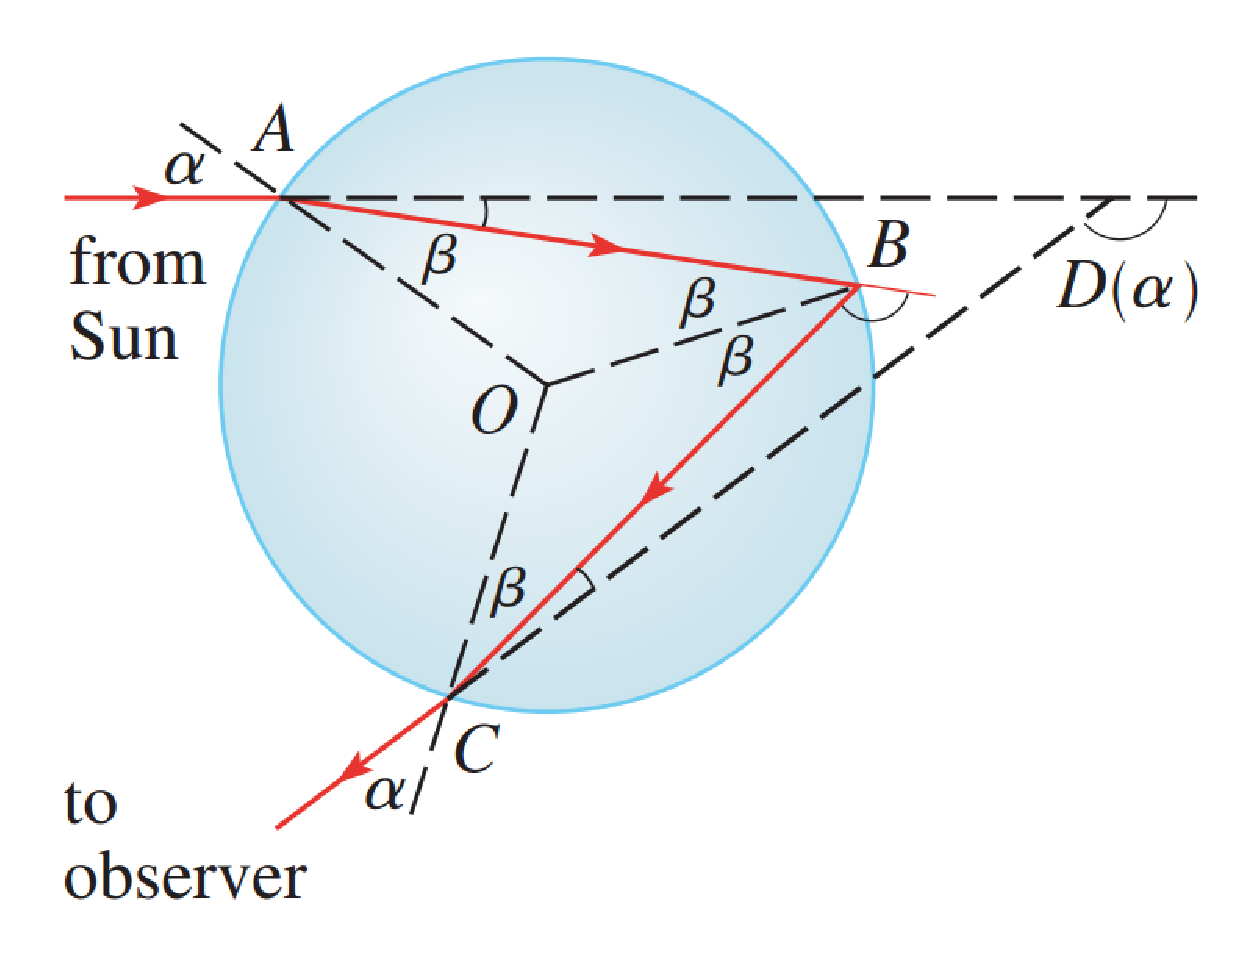
\includegraphics[scale=0.35]{activities/math112/figures/Rainbow.eps}
	\caption{Formation of the primary rainbow.}
	\label{fig:rainbow1}
\end{figure}

Figure \ref{fig:rainbow1} shows a ray of sunlight entering a spherical raindrop at $A$. Some of the light is reflected, but the line $AB$ shows the path of the part that enters the drop. Notice that the light is refracted toward the normal line $AO$ and in fact Snell's Law says that 
\begin{equation}
\label{eq:snellslaw}
\sin(\alpha)=k\sin(\beta),
\end{equation}
\index{mathematical functions!sine}
where $\alpha$ is the angle of incidence, $\beta$ is the angle of refraction, and $k \approx \frac{4}{3}$ is the index of refraction for water. At $B$, some of the light passes through the drop and is refracted into the air, but the line $BC$ shows the part that is reflected. 

\subsection*{Exercises:}
\begin{enumerate}
\item When the ray reaches $C$, part of it is reflected, but for the time being we are more interested in the part that leaves the raindrop at $C$. The angle of deviation $D(\alpha)$\index{greek letter!alpha}\index{greek letter!beta} is the amount of clockwise rotation that the ray has undergone during this three-stage process. The formula for the angle of deviation is given by
\marginnote{The Greek letters alpha ($\alpha$) and beta ($\beta$) can be found on the Greek palette, or typed out and autocompleted using ESC or Ctrl+Space.}
\begin{equation}
\label{eq:deviation1}
D(\alpha)=\pi + 2\alpha -4\beta.
\end{equation}
\clearpage
    \begin{enumerate}
    \marginnote{Make sure to use a lower case $d(\alpha)$ instead of $D(\alpha)$. Maple uses $D$ as a shorthand command for derivatives.}
    \item Solve Equation \eqref{eq:snellslaw} for $\beta$ and substitute this into Equation \eqref{eq:deviation1}.
    \item Show that the minimum value of the deviation is $D(\alpha) \approx 138^{\circ}$ and occurs when $\alpha \approx 59.4^\circ$. 
    \item Plot the Angle of Deviation function in Maple to verify your answer to (b). 
    \end{enumerate}
    \marginnote[-1cm]{You may use the closed interval method over the interval $\alpha \in \left[0,\tfrac{\pi}{2}\right]$. Note that Maple will give you answers in radians, so you will have to convert to degrees. }
\end{enumerate}

The significance of the minimum deviation is that when $\alpha \approx 59.4^\circ$, we have $D'(\alpha)\approx 0$, so $\Delta D/\Delta \alpha \approx 0$. This means that many rays with $\alpha \approx 59.4^\circ$ become deviated by approximately the same amount. It is the concentration of rays coming from near the direction of minimum deviation that creates the brightness of the primary rainbow. Figure \ref{fig:rainbow2} shows that the angle of elevation from the observer up to the highest point on the rainbow is $180^\circ - 138^\circ=42^\circ$. (This angle is called the rainbow angle.) The rainbow angle is found by subtracting the angle of deviation from $180^\circ$ (i.e. $180^\circ - D(\alpha)$).
\marginnote[-2cm]{The rainbow angle is found by \[180^\circ - D(\alpha).\]}
    
\begin{figure}[h]
	\centering
	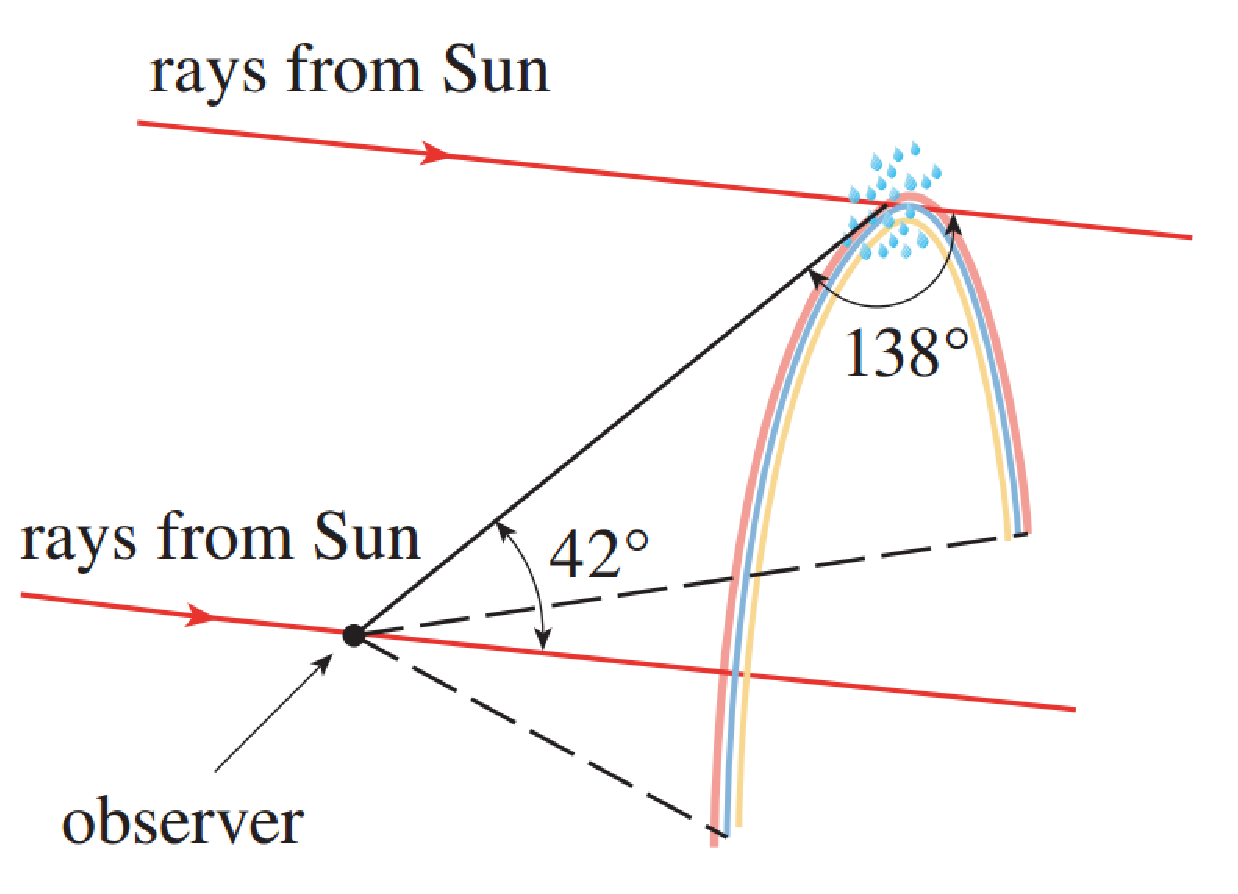
\includegraphics[scale=0.25]{activities/math112/figures/Rainbow2.eps}
	\caption{Angle of elevation from observer.}
	\label{fig:rainbow2}
\end{figure}

Exercise 1 explains the location of the primary rainbow, but how do we explain the colours? Sunlight comprises a range of wavelengths, from the red range through orange, yellow, green, blue, indigo, and violet (ROYGBIV! Ring a bell?). As Newton discovered in his prism experiments of $1666$, the index of refraction is different for each colour. (The effect is called dispersion.)

\begin{enumerate}
\setcounter{enumi}{1}
	\item For red light, the refractive index is $k \approx 1.3318$, whereas for violet light it is $k \approx 1.3435$. By repeating the calculation of exercise 1 for these values of $k$, show that the rainbow angle is about $42.3^\circ$ for the red bow and $40.6^\circ$ for the violet bow. So the rainbow really consists of seven individual bows corresponding to the seven colours.
	\marginnote[-3cm]{In this example, you will repeat exercise 1 using different refractive indices of different colours of light.}
\end{enumerate}

Perhaps you have seen a fainter secondary rainbow above the primary bow. That results from the part of a ray that enters a raindrop and is refracted at $A$, reflected twice (at $B$ and $C$), and refracted as it leaves the drop at $D$ (see Figure \ref{fig:rainbow3}). 
	
\begin{figure}[h]
	\label{fig:rainbow3}
	\centering
	\parbox{0.5\linewidth}{
		\includegraphics[scale=0.25]{activities/math112/figures/Rainbow3.eps}
		\caption{Formation of the secondary rainbow.}
	}
	\hspace{0.05\linewidth}
	\parbox{0.4\linewidth}{
		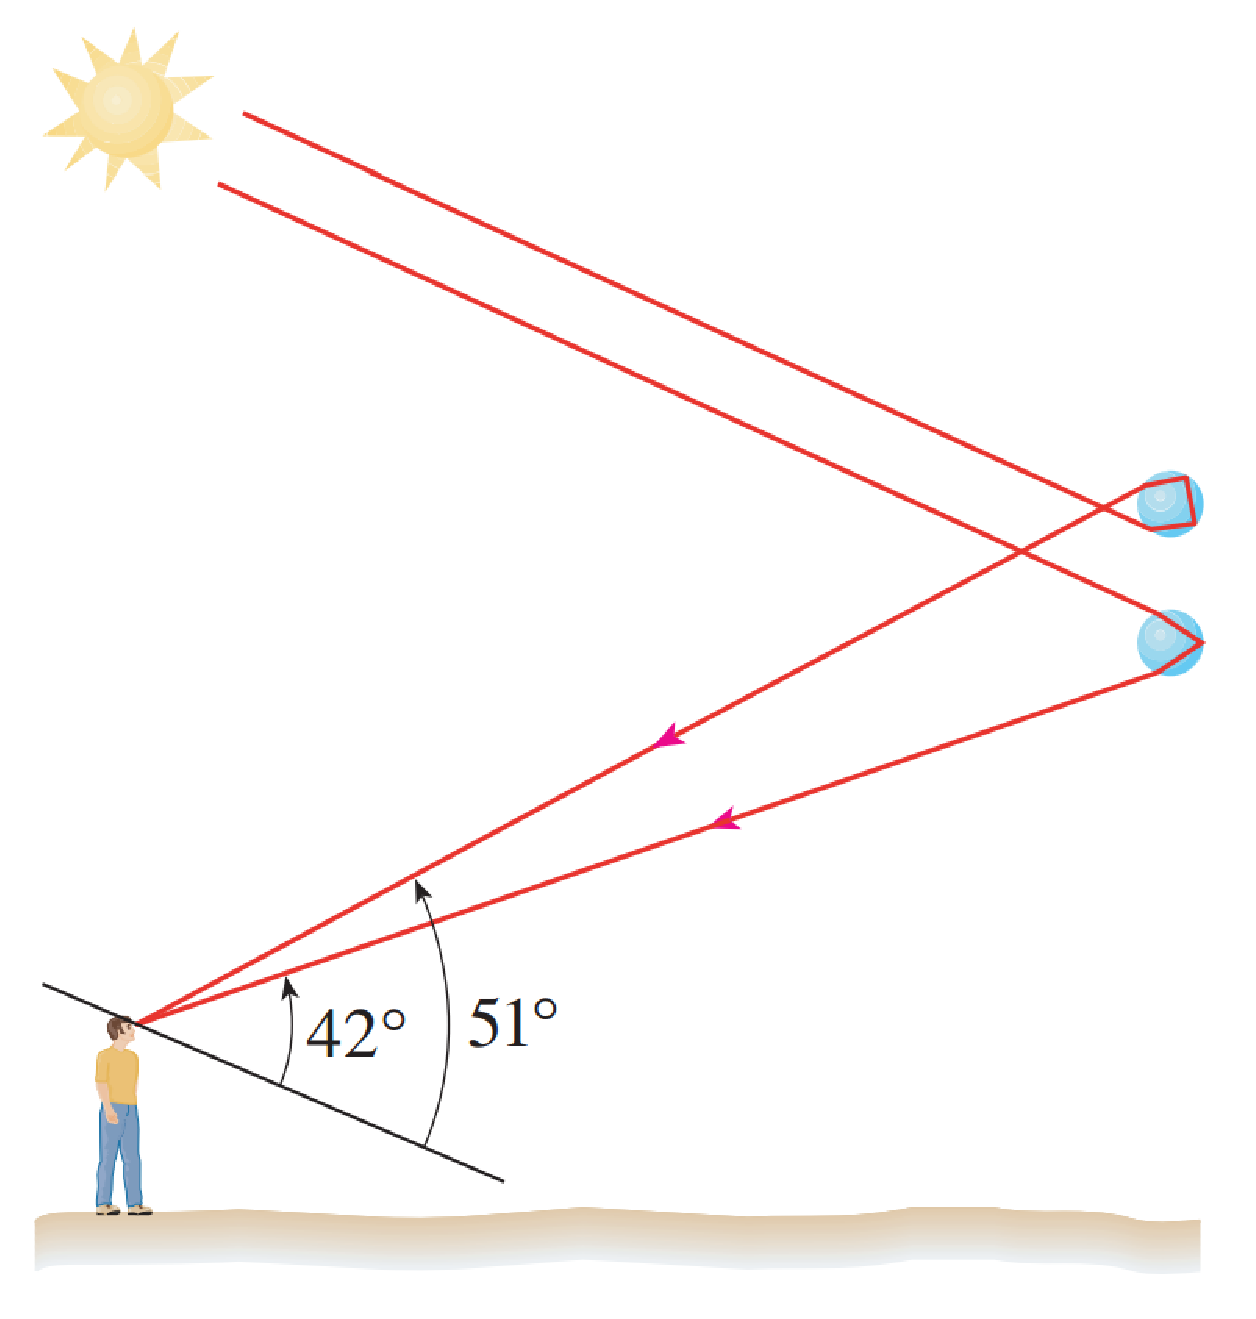
\includegraphics[scale=0.25]{activities/math112/figures/Rainbow4.eps}
		\caption{Angles of elevation from observer.}
	}
\end{figure}

\begin{enumerate}
\setcounter{enumi}{2}	
	\item This time the deviation angle $D(\alpha)$ is the total amount of counterclockwise rotation that the ray undergoes in this four-stage process. In this case, the angle of deviation is given by the formula
\begin{equation}
\label{eq:deviation2}
D(\alpha)=2\alpha-6\beta+2\pi,
\end{equation}
and $D(\alpha)$ has a minimum value when 
\begin{equation}
\label{eq:minvalue}
\cos(\alpha)=\sqrt{\dfrac{k^2-1}{8}}.
\end{equation} \index{mathematical functions!cosine}

\marginnote{It is still necessary to use Snell's Law (Equation \eqref{eq:snellslaw}) to determine the angle of deviation: \[\sin(\alpha)=k\sin(\beta)\]}
	\begin{enumerate}
	\item Solve Equation \eqref{eq:snellslaw} for $\beta$ and substitute this into Equation \eqref{eq:deviation2}. 
	\item When $k \approx \frac{4}{3}$, find the angle of incidence, $\alpha$, using Equation \eqref{eq:minvalue}.
	\item Find the angle of deviation, $D(\alpha)$, using your answers from exercises 3(a) and 3(b).
	\item Verify that the rainbow angle for the secondary rainbow is approximately $51^\circ$, as shown in Figure \ref{fig:rainbow3}.
	\marginnote[-0.5cm]{The rainbow angle is found by \[180^\circ - D(\alpha).\]}
	\end{enumerate}
\end{enumerate}
	

%\subsection*{Notes:}
%\begin{itemize}
%    \item   Use 15 decimal places to find your answers, when applicable.
    
 
%\end{itemize}